
\documentclass[12pt,a4paper]{article}
\usepackage{times}
\usepackage{durhampaper}
\usepackage{harvard}
\usepackage{graphicx}

\citationmode{abbr}
\bibliographystyle{agsm}

\title{Implementation and Analysis of an Elliptic Curve Cryptography System with Safe Curves}
\author{} % leave; your name goes into \student{}
\student{T. Butterfield}
\supervisor{M. Bordewich}
\degree{BSc Computer Science}

\date{\today}

\begin{document}

\maketitle

\begin{abstract}
Do not cite references in the abstract.

This section should not be longer than half of a page, and having no more than one or two sentences under each heading is advised.

\paragraph{Background} -
Diffie-Hellman, RSA, ...

\paragraph{Aims} -
Create system implementing ECC safe curves
The aim of this project was to create a working Elliptic Curve Cryptography system 
and to analyse that system in terms of security and efficiency. 

\paragraph{Method} -
Euclid's extended algorithm, point addition, point multiplication, ...

\paragraph{Results} -
Cannot discover information about private key, enables secure communication

\paragraph{Conclusions} -
Strength of ECC, smaller key size than RSA, much more suitable for mobile devices

\end{abstract}


\begin{keywords}
Elliptic Curve Cryptography (ECC), Elliptic Curve Diffie-Hellman (ECDH), Elliptic Curve Digital Signature Algorithm (ECDSA), 
Safe Curves, User Interface (UI)
\end{keywords}


\section{Introduction}
The whole report, including references, should not be longer than 20 pages in length.
It should be noted that not all the details of the work carried out in the project can be represented in 20 pages.
It is therefore vital that the Project Log book be kept up to date as this will be used as supplementary material when the project paper is marked.
There should be between 10 and 20 referenced papers---references to Web based pages should be less than 10\%.

This section briefly introduces the general project background, the research question you are addressing, and the project objectives.
It should be between 2 to 3 pages in length.

- Abstract \& Introduction make 5\% of paper

- Adequacy of Abstract

- Description of background - Diffie-Hellman, RSA, ECC

- Discussion of aims and achievements - Aimed to create system which implemented safe curves 

There were a total of nine objectives for this project, split equally into three sections: basic, intermediate, and advanced. 

The first basic objective was to create a basic working ECC system which computed the essential functions required. 
The second and third basic objectives were to create a client application that can conduct ECDH over a network connection, 
and to create a UI allowing a user to easily make use of the system and to decide what level of complexity is revealed to them. 

The intermediate objectives revolved around improving the functionality and security of the system, 
with the first objective being to add secure random private key generation to the system. 
The other intermediate objectives were to implement the ECDSA and to enable the exchange of secure signed files via the UI. 

The first advanced objective was to make improvements to the UI and to reveal the workings of the system. 
The penultimate objective was to analyse the code for efficiency, including how the time required scales with the curve and key size, 
making any necessary changes to the system to improve the efficiency. 
The final objective was to analyse the code for vulnerabilities, such as side-channel attacks, and to fix any such weaknesses. 


\section{Related Work}
This section presents a survey of existing work on the problems that this project addresses. 
it should be between 2 to 4 pages in length. 

- 15\% of paper

- Adequacy of literature surveyed

- Critical analysis

Cryptography is the study of mathematical systems for solving two kinds of security problems: privacy and authentication \cite{1055638}. 
A privacy system prevents the extraction of information by unauthorised parties from messages transmitted over a public channel, assuring it is read only by the intended recipient. 
An authentication system prevents the unauthorised injection of messages into a public channel, assuring the legitimacy of the sender. 
\cite{1055638} proposed that it was possible to develop systems in which two parties communicating solely over a public channel and using only publicly known techniques could create a secure connection. 
This was the first public discovery of public-key cryptography.

Diffie and Hellman presented the concept of a public-key cryptosystem but not any practical implementation of such a system. 
So in 1978, Rivest, Shamir, and Adleman presented a new encryption method which did just that, it was the first public implementation of public-key cryptography. 
This method had the novel property that publicly revealing an encryption key did not thereby reveal the corresponding decryption key \cite{10.1145/359340.359342}. 
This is known as RSA public-key cryptography. 

\cite{10.1007/3-540-39799-X_31} and \cite{koblitz1987elliptic} discussed an analogue of the Diffie-Hellman key exchange protocol based on elliptic curves over finite fields which used the multiplicative group of a finite field. 
The advantage of this system was that it appeared to be immune from attacks of the style of \cite{10.1007/3-540-39799-X_31,4568001}. 
This was the invention of Elliptic Curve Cryptography. 

Whilst the \emph{Elliptic Curve Discrete Logarithm Problem} is difficult to solve on classical computers \cite{hankerson2003guide}, 
there is a gap between ECDLP difficulty and ECC security \cite{bernstein2013safecurves}. 
In 2010, it was discovered that Sony had made a basic and critical mistake in the implementation of their Elliptic Curve Cryptosystem. 
As discussed in section \ref{Signature Generation}, as part of the Signature Generation stage of the ECDSA, a random integer $k$ is generated and used, 
it is imperative that $k$ is truly random and not predictable in any way. 
However, Sony wrote their own software which used a constant number for each signature. 
This allowed the computation of their private key, from the public key, using simple algebra \cite{hotz2010console}.


\section{Solution}
This section presents the solutions to the problems in detail. 
The design and implementation details should all be placed in this section. 
You may create a number of subsections, each focussing on one issue.  

This section should be between 4 to 7 pages in length.

- 25\% of paper

- Adequacy of the solution - 

- Specification and design - written in python, command line interface

- Outline of implementation issues - issues with communicating over a network, client instances must be on same local device

- Description of tools used - various python libraries: Pyro4, AES, base64, hashlib, secrets

- Verification and Validation - 

- Discussion of testing - Graphs from testing of security and efficiency of system: number of 1 bits vs time, log key value vs time, various curves vs time.

\subsection{Point Arithmetic} \label{Point Arithmetic}
The addition operation in $E(F_p)$ is specified as follows:

\subsubsection{Point Addition} \label{Point Addition}
Let $P = (x_1,y_1) \in E(F_p)$ and $Q = (x_2,y_2) \in E(F_p)$, where $P \neq Q$. 
Then $P + Q = (x_3,y_3)$, where
\begin{equation}
    x_3 = \lambda^2 - x_1 - x_2, \quad y_3 = \lambda(x_1 - x_3) - y_1, \quad and \quad \lambda = \frac{y_2-y_1}{x_2-x_1}
\end{equation}

\subsubsection{Point Doubling} \label{Point Doubling}
Let $P = (x_1,y_1) \in E(F_p)$. 
Then $P + P = 2P = (x_3,y_3)$, where
\begin{equation}
    x_3 = \lambda^2 - 2x_1, \quad y_3 = \lambda(x_1 - x_3) - y_1, \quad and \quad \lambda = \frac{3x_1^2 + a}{2y_1}
\end{equation}
\cite{lopez2000overview}.

\subsection{Protocols} \label{Protocols}
In cryptography it is customary to personalise the participants. 
Typically, Alice and Bob want to communicate, while Eve, the eavesdropper, 
intercepts and tries to read their messages \cite{silverman2009arithmetic}.

The EC algorithms are specified in \emph{SEC 1: Elliptic Curve Cryptography} \cite{brown2009standards}. 
An overview of EC cryptographic algorithms for key agreement and digital signature are explained below.

\subsubsection{ECDH} \label{ECDH}
The \emph{Elliptic Curve Diffie-Hellman} key agreement protocol allows Alice and Bob 
to securely exchange the value of a point on an elliptic curve, 
although neither of them initially knows the value of the point \cite{anoop2007elliptic,silverman2009arithmetic}: 
Alice and Bob must agree on a finite field $F_q$, an elliptic curve $E/F_q$, and a generator point $G \in E(F_q)$  of (prime) order $n$.
Both Alice and Bob have a key pair $(d,Q)$ consisting of a private key $d$ (a randomly selected integer less than $n$) 
and a public key $Q = d * G$.

Let $(d_A,Q_A)$ be the key pair of Alice and $(d_B,Q_B)$ be the key pair of Bob.

1. Alice computes $K = (x_K,y_K) = d_A * Q_B$

2. Bob computes $L = (x_L,y_L) = d_B * Q_A$

3. Since $d_AQ_B = d_Ad_BG = d_Bd_AG = d_BQ_A$. Therefore $K = L$ and hence $x_K = x_L$

4. Hence the shared secret is $x_K$

Since it is practically impossible to find the private key $d_A$ or $d_B$ from the public key $K$ or $L$, it is not possible for Eve to obtain the shared secret \cite{anoop2007elliptic,silverman2009arithmetic,jurivsic1997elliptic}.

\subsubsection{ECDSA} \label{ECDSA}
The \emph{Elliptic Curve Digital Signature Algorithm} allows Alice to sign a digital document and Bob to verify that the signature is valid \cite{silverman2009arithmetic}:
To authenticate a message sent by Alice, she signs the message using her private key. 
Alice sends the message and the signature to Bob. 
This signature can be verified only by using the public key of Alice. 
Since Bob knows Alice's public key, he can verify whether the message was indeed sent by Alice or not \cite{anoop2007elliptic}.
ECDSA is a variant of the Digital Signature Algorithm (DSA) that operates on elliptic curve groups. 

Alice and Bob must first agree on a finite field $F_p$, an elliptic curve $E/F_p$, and a generator point $G \in E(F_p)$ of (prime) order $n$.
Sender Alice has a key pair $(d_A,Q_A)$ consisting of a private key $d_A$ (a randomly selected integer less than $n$) 
and a public key $Q_A = d_A * G$ ($G$ is the generator point). 
An overview of the ECDSA process is defined below. 

\subsubsection{Signature Generation} \label{Signature Generation}
For signing a message $m$ sent by Alice, using Alice's private key $d_A$.

1. Calculate $e = HASH(m)$, where $HASH$ is a cryptographic hash function, such as SHA

2. Select a random integer $k$ from $[1,n-1]$

3. Calculate $r = x1$ (mod $n$), where $(x1,y1) = k * G$. If $r = 0$, go to step 2

4. Calculate $s = k^{-1}(e+d_Ar)$ (mod $n$). If $s = 0$, go to step 2

5. The signature is the pair $(r,s)$ \cite{hankerson2003guide,anoop2007elliptic,koblitz2000state,silverman2009arithmetic,jurivsic1997elliptic}.

\subsubsection{Signature Verification} \label{Signature Verification}
For Bob to authenticate Alice's signature, Bob must have Alice's public key $Q_A$.

1. Verify that $r$ and $s$ are integers in $[1,n-1]$. If not, the signature is invalid

2. Calculate $e =HASH(m)$ where $HASH$ is the same function used in the signature generation (Section \ref{Signature Generation}).

3. Calculate $w = s^{-1}$ (mod $n$)

4. Calculate $u_1 = ew$ (mod $n$) and $u_2 = rw$ (mod $n$)

5. Calculate $(x1,y1) = u_1G + u_2Q_A$

6. The signature is valid if $x1 = r$ (mod $n$), invalid otherwise \cite{hankerson2003guide,anoop2007elliptic,koblitz2000state,silverman2009arithmetic,jurivsic1997elliptic}.

\subsection{Safe Curves} \label{Safe Curves}
There are several different standards covering selection of curves for use in elliptic-curve cryptography: 
\begin{itemize}
    \item ANSI X9.62 (1999)
    \item IEEE P1363 (2000)
    \item SEC 2 (2000)
    \item NIST FIPS 186-2 (2000)
    \item ANSI X9.63 (2001)
    \item Brainpool (2005)
    \item NSA Suite B (2005)
    \item ANSSI FRP256V1 (2011)
\end{itemize}
Each of these standards tries to ensure that the ECDLP (finding a user's private key, given their public key) is difficult. 
Unfortunately, there is a gap between ECDLP difficulty and ECC security. 
None of these standards do a good job of ensuring ECC security, 
secure implementations of the standard curves are theoretically possible but very hard. 
There are many attacks that break real-world ECC without solving ECDLP \cite{bernstein2013safecurves}. 
MORE DETAIL ABOUT WHAT MAKES A CURVE SAFE/UNSAFE

In 2006, Daniel Bernstein designed a new high-security ECDH function which achieved record setting speeds (twice as fast as any other function), 
with several side benefits including state-of-the-art timing-attack protection. 
This function, known as Curve25519, is suitable for a wide variety of cryptographic applications. 
The Curve25519 function is $F_p$-restricted x-coordinate scalar multiplication on $E(F_{p^2})$, 
where $p$ is the prime number $2^{255} - 19$ and $E$ is the elliptic curve $y^2 = x^3 + 486662x^2 + x$ \cite{10.1007/11745853_14}.
Curve25519 is regarded as a safe curve, since it satisfies the basic parameter requirements, the ECDLP security requirements, 
and the ECC security requirements beyond ECDLP security \cite{bernstein2013safecurves}.

\subsection{Exhaustive Search} \label{Exhaustive Search}
The elliptic curve parameters for cryptograhic schemes should be carefully chosen in order to resist all known attacks on the ECDLP. 
The most na\"{\i}ve algorithm for solving the ECDLP is exhaustive search whereby one computes the sequence of points $P,2P,3P,4P,...$ until $Q$ is encountered. 
The running time is approximately $n$ steps in the worst case and $n/2$ steps on average. 
Therefore, exhaustive search can be circumvented by selecting elliptic curve parameters with $n$ sufficiently large to represent an infeasible amount of computation (e.g., $n \geq 2^{80}$) \cite{hankerson2003guide}.

\subsection{Pohlig-Hellman and Pollard's rho algorithm} \label{Pohlig-Hellman and Pollard's rho algorithm}
The best general-purpose attack known on the ECDLP is the combination of the Pohlig-Hellman algorithm and Pollard's rho algorithm, 
which has a fully-exponential running time of $O( \sqrt p \,)$ where $p$ is the largest prime divisor of $n$. 
To resist this attack, the elliptic curve parameters should be chosen so that $n$ is divisible by a prime number $p$ sufficiently large 
so that $\sqrt p$ steps is an infeasible amount of computation (e.g., $p > 2^{160}$).
If, in addition, the elliptic curve parameters are carefully chosen to defeat all other known attacks (e.g. Isomorphism attacks), 
then the ECDLP is believed to be infeasible given the state of today's computer technology \cite{hankerson2003guide}.

\subsection{Testing}
I analysed the time taken to compute $kG$ here and Figure \ref{fig:curves} shows the results
\begin{figure}[htb]
    \centering
    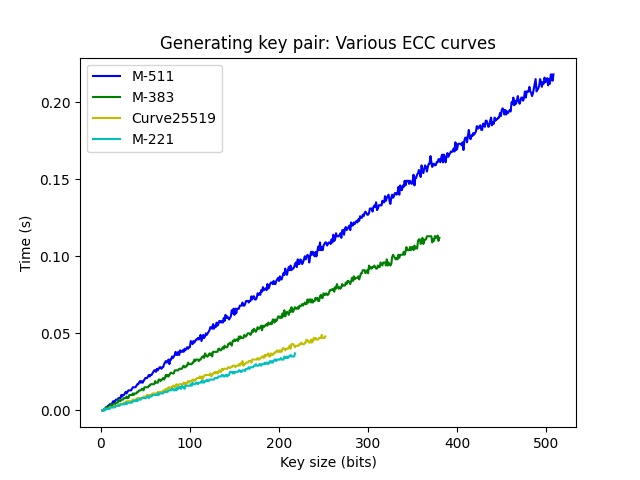
\includegraphics[width=0.5\textwidth]{figures/Timing.png}
    \caption{Comparison of various safe curves}
    \label{fig:curves}
\end{figure}

I also looked at whether my implementation leaks any information through timing attacks, 
for example, is it possible to determine how many 1s are in the binary expansion of the key by analysing the time taken to compute 
results in Figure \ref{fig:number1s}. 
\begin{figure}[htb]
    \centering
    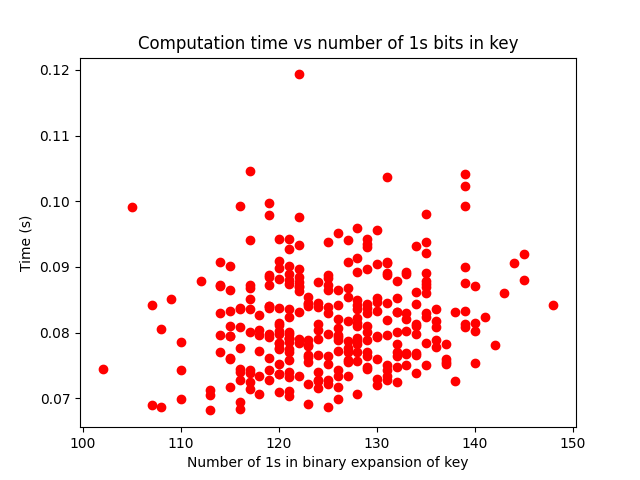
\includegraphics[width=0.5\textwidth]{figures/ones300SmoothedAny.png}
    \caption{Analysis of information leaked through timing attacks}
    \label{fig:number1s}
\end{figure}

I then investigated timing attacks with regards to the size of the binary expansion of the key in Figure \ref{fig:logbase2}
\begin{figure}[htb]
    \centering
    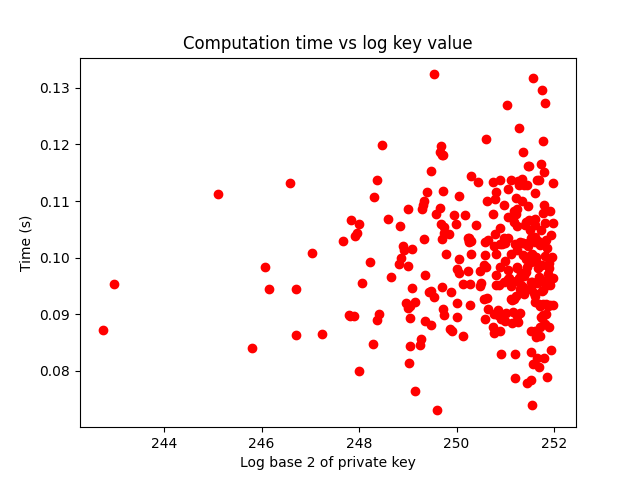
\includegraphics[width=0.5\textwidth]{figures/keyValue300SmoothedAny.png}
    \caption{Timing attacks analysis}
    \label{fig:logbase2}
\end{figure}


\section{Results}
This section presents the results of the solutions. 
It should include information on experimental settings. 
The results should demonstrate the claimed benefits/disadvantages of the proposed solutions.

This section should be between 2 to 3 pages in length.

- 25\% of paper

- Description of the evaluation method adopted - evaluated by trying to break the encryption and demonstrating that it would take an infeasible amount of time

- Clarity of results


\section{Evaluation}
This section should between 1 to 2 pages in length.

- 20\% of paper

- Suitability of approach

- Discussion of strengths and limitations of the system - limitations with communicating over networks, works well with multiple client instances on a local machine

- Discussion of algorithms used - ECDH, ECDSA, point addition and point multiplication

- Appraisal of project organisation


\section{Conclusions}
This section summarises the main points of this paper. 
Do not replicate the abstract as the conclusion. 
A conclusion might elaborate on the importance of the work or suggest applications and extensions. 
This section should be no more than 1 page in length. 

- 5\% of paper

- Description of the main findings

- Clarity of conclusions

- Discussion of further work

Much research has been done into Elliptic Curve Cryptography since its discovery in 1985 \cite{10.1007/3-540-39799-X_31,koblitz1987elliptic}. 
The security of ECC is based on the hardness of the ECDLP, 
and currently the best algorithms known to solve the ECDLP have fully exponential running time. 
In contrast to the subexponential-time algorithms known for the integer factorisation problem, 
on which the security of RSA is based. 
This means that, for example, a 160-bit EC key provides the same level of security as a 1024-bit RSA key \cite{hankerson2003guide,silverman2009arithmetic}. 
ECC is a very strong encryption method, but only when implemented properly, 
using a safe curve \cite{bernstein2013safecurves,10.1007/11745853_14}
and a good random number generator \cite{hotz2010console}. 


\bibliography{projectpaper}


\end{document}
